\PassOptionsToPackage{unicode,pdfusetitle}{hyperref}
\PassOptionsToPackage{hyphens}{url}

\documentclass{article}
\usepackage[a4paper,includeheadfoot,top=1cm,bottom=1cm,left=2cm,right=1cm]{geometry}
\usepackage{amsmath,amssymb}
\usepackage{fontspec}
\usepackage[russian]{babel}
\usepackage{microtype}
\usepackage{parskip}
\usepackage{xcolor}
\definecolor{navy}{RGB}{0,0,128}
\setmainfont{Noto Serif}
\setsansfont{Monitorica}
\setmonofont{Noto Sans Mono}
\newfontfamily\headingfont{Operation Napalm}
\usepackage{titlesec}
\titleformat{\section}{\headingfont\color{navy}\Large}{\thesection}{1em}{}[\titlerule]
\titleformat{\subsection}{\headingfont\color{navy}\large}{\thesubsection}{1em}{}
\titleformat{\subsubsection}{\headingfont\color{navy}\normalsize}{\thesubsubsection}{1em}{}
\titleformat{\paragraph}{\headingfont\color{navy}\normalsize}{\theparagraph}{1em}{}
\titleformat{\subparagraph}{\headingfont\color{navy}\normalsize\itshape}{\thesubparagraph}{1em}{}
\usepackage{multicol}
\usepackage{array}
\usepackage{wallpaper}
\usepackage{background}
\usepackage{tabularray}
\usepackage{tblr-extras}
\usepackage{multirow}
\usepackage{makecell}
\usepackage{calc}
\usepackage{rotating}
\usepackage{caption}
\usepackage{capt-of}
\usepackage{titletoc}
\usepackage{graphicx}
\usepackage{wrapfig}
\UseTblrLibrary{booktabs,caption,babel}
\makeatletter
\def\maxwidth{\ifdim\Gin@nat@width>\linewidth\linewidth\else\Gin@nat@width\fi}
\def\maxheight{\ifdim\Gin@nat@height>\textheight\textheight\else\Gin@nat@height\fi}
\makeatother
\setlength{\emergencystretch}{3em}
\providecommand{\tightlist}{
  \setlength{\itemsep}{0pt}\setlength{\parskip}{0pt}}
\providecommand{\fillinline}[1]{%
  \leavevmode\leaders\hbox to 0.5556em{\hss.\hss}\hfill\kern0pt}
\setcounter{secnumdepth}{5}
\setcounter{tocdepth}{5}
\titlecontents{section}[0em]{}{\Large\makebox[1.3em][l]{\thecontentslabel}}{}{\titlerule*[0.8pc]{.}\contentspage}
\titlecontents{subsection}[0em]{}{\large\makebox[2.1em][l]{\thecontentslabel}}{}{\titlerule*[0.8pc]{.}\contentspage}
\titlecontents{subsubsection}[0em]{}{\makebox[3.2em][l]{\thecontentslabel}}{}{\titlerule*[0.8pc]{.}\contentspage}
\titlecontents{paragraph}[0em]{}{\small\makebox[4.2em][l]{\thecontentslabel}}{}{\titlerule*[0.8pc]{.}\contentspage}
\titlecontents{subparagraph}[0em]{}{\footnotesize\makebox[5.0em][l]{\thecontentslabel}}{}{\titlerule*[0.8pc]{.}\contentspage}
\usepackage{bookmark}
\IfFileExists{xurl.sty}{\usepackage{xurl}}{}
\urlstyle{same}
\hypersetup{
  hidelinks
}

\captionsetup{labelfont={it,color=navy},textfont={it,color=navy},justification=centering}
\captionsetup[table]{hypcap=false}
\captionsetup[figure]{hypcap=false}
\addto\extrasrussian{
  \def\tableautorefname{Таблица}
  \def\figureautorefname{Схема}
  \def\sectionautorefname{Раздел}
  \def\subsectionautorefname{Подраздел}
  \def\subsubsectionautorefname{Параграф}
  \def\paragraphautorefname{Абзац}
  \def\pageautorefname{Страница}
  \def\equationautorefname{Формула}
}

\title{Мир и процветание}
\newcommand{\siteurl}{https://vk.com/playingwar}
\author{Никита Макаров}

\begin{document}
\begin{titlepage}

\backgroundsetup{
  scale=1,
  angle=0,
  opacity=1,
  position={current page.center},
  contents={
\includegraphics[width=\paperwidth,height=\paperheight,clip]{media/pap_players_book/image2.png}}
}

\begin{center}
\vspace*{2cm}

{\color{navy}\fontsize{48}{56}\selectfont\textbf{Мир и процветание}}

\vspace{0.5cm}

{\color{navy}\fontsize{32}{40}\selectfont\textbf{Журнал игрока}}

\vfill

{\color{white}\Large\textbf{Никита Макаров}}

{\color{white}\href{\siteurl}{\textbf{\MakeUppercase{\siteurl}}}}

{\color{white}\textbf{Санкт-Петербург}}

\end{center}
\end{titlepage}

\clearpage

\backgroundsetup{
  scale=1,
  angle=0,
  opacity=1,
  position={current page.center},
  contents={\TileWallPaper{1cm}{1cm}{media/common/image1.jpg}}
}

\begin{multicols}{2}
\raggedcolumns{}

\renewcommand{\contentsname}{Содержание}
\tableofcontents
\thispagestyle{empty}

\clearpage

\section{Введение}\label{intro}

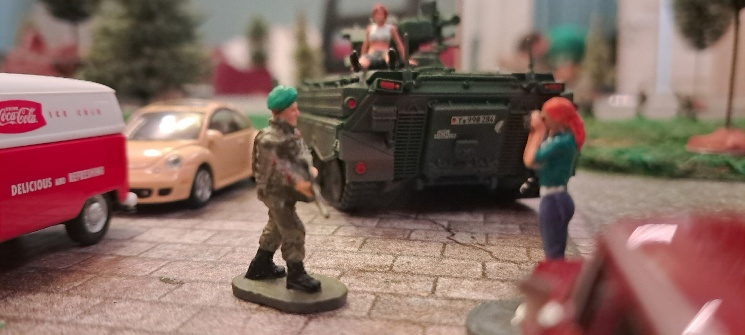
\includegraphics[width=\linewidth]{media/pap_players_book/image3.jpeg}

Вашему вниманию предлагается модуль к игре Контракт. Модуль рассчитан примерно на 24--32 часа и создан таким образом, чтобы плавно познакомить игроков с системой, навыками и основными механиками, используемыми в игре.

Действие происходит в наше время в альтернативной реальности. Крупная международная компания <<Мир и процветание>> заключает договор с правительством Белиза о предоставлении услуг в области охраны правопорядка и обороны страны. Договор предусматривает поэтапный переход функций от армии и полиции к компании <<Мир и процветание>> с последующим расформированием государственных структур, но для этого компании предстоит доказать свою эффективность в течение переходного периода.

Не все довольны этой ситуацией. Некоторые кадровые офицеры армии и полиции Белиза опасаются, что потеряют своё влияние, доход и положение в обществе. Националисты из разных слоёв общества воспринимают приход транснациональной компании как нарушение суверенитета и готовы противостоять ей любыми средствами. Некоторые просто пользуются ситуацией и возможностями, открывающимися из-за неизбежных накладок во время переходного периода, для личного обогащения.

Компания <<Мир и процветание>> нанимает людей для работы в Белизе через сеть своих офисов в разных странах\dots

\section{Персонажи и отряды}\label{units}

Как и в других настольных ролевых играх, вам, как игроку, будет предложено отождествить себя с вымышленным персонажем,
которого вы можете придумать сами. Этот персонаж может быть вашим клоном в игровом мире, либо совершенно другим человеком, в
роль которого вы можете вжиться. Это может быть даже человек другого пола, с другими ценностями, с другими физическими особенностями.

Однако, ваш персонаж не является неуязвимым супергероем, обладающим сверхчеловеческими способностями. Это обычный человек,
хотя, возможно, и обладающий некоторыми навыками на пределе человеческих возможностей. Поэтому \textbf{вашей игровой фишкой будет не
один ваш персонаж, а целый отряд}, который вы соберёте. Это существенное отличие этой игры от самых популярных
современных настольных ролевых игр, таких как Dugneons \& Dragons, и больше похоже на компьютерные реализации D\&D, такие как, например,
Might and Magic, Baldur's Gate, Icewind Dale и так далее.

\begin{wrapfigure}{r}{3cm}
  
\includegraphics[height=3.5cm]{media/pap_players_book/image8.png}
\end{wrapfigure}
{\color{navy}
\emph{--- Но скажи мне, Джек, чьи это молодцы идут за нами?\\
--- Мои, Хел, мои.\\
--- Никогда в жизни я не видал такого жалкого сброда.\\
--- Ба! Они достаточно хороши, чтобы истыкать их копьями. Пушечное мясо, пушечное мясо!
Они заполнят могилу не хуже других. Смертные люди, братец ты мой, смертные люди!}

\rightline{\textbf{Уильям Шекспир, <<Генрих IV, часть 1>>}}}

Именно \textbf{отряд вам предстоит <<прокачивать>>, правильно подбирая комбинацию характеристик персонажей и снаряжения} так, чтобы они дополняли
друг-друга. У каждого отряда должен быть лидер, который мог бы вдохновлять и организовывать своих людей. В игре у отдельных персонажей нет
<<хит пойнтов>>, как и в реальной жизни, но для отряда в качестве <<хит пойнтов>> может служить количество персонажей в отряде.

Современное вооружение отличается дальнобойностью и могуществом. Человеку достаточно одной пули или осколка, чтобы погибнуть,
и даже танку достаточно одного хорошего попадания, чтобы быть полностью уничтоженным. Даже опытнейший ветеран спецназа погибнет,
если выйдет на бой в одиночку, не создав для себя выгодные условия. Бои выигрываются тактически, для чего необходимо собрать команду,
грамотно организовать управление, составить план и распределить роли.

Игра поощряет желание персонажа и игрока стать лидером, который возьмёт ответственность за свой отряд, снабдит его всем необходимым
для выполнения задачи и постарается избежать потерь. Тщательная подготовка к бою является ключом к этому. Любая задача должна начинаться
с решения вопроса снабжения. К этому вопросу следует подходить творчески, искать и использовать неявные ресурсы, чтобы получить преимущество.

Важно с умом подходить к формированию отрядов, нужно понимать задачу для отряда и подбирать людей в него под задачу. Один новичок в
разведывательной группе, не умеющий маскироваться, может подставить под огонь всю группу. Один слабый боец в отряде,
который должна совершить марш-бросок, будет тормозить весь отряд. Отряд без лидера или со слабым лидером в критический момент может
замешкаться из-за недопонимания.

\begin{wrapfigure}{l}{3cm}
  
\includegraphics[height=4cm]{media/pap_players_book/image7.png}
\end{wrapfigure}
{\color{navy}
\emph{\\\\\\\\\\\\\\\\\\\\Цепь так же крепка, как и её самое слабое звено.}

\rightline{\textbf{Английская пословица}}}

Вряд ли стоит напоминать о базовых тактиках, вроде разделения отрядов на огневую и штурмовую группы, использовании дымовых шашек,
окружении противника и отрезании ему путей отхода. О чём стоило бы упомянуть, так это о скрытности и стрессе.
Необходимо стараться скрытно занимать выгодные позиции, стараться обнаружить противника прежде, чем открывать огонь, и при этом помнить,
что открытие огня непременно выдаст ваше местоположение противнику. Вместе с этим, при штурме следует использовать любую возможность
вести подавляющий огонь по позициям противника, чтобы подойти к нему ближе и, возможно, даже взять в плен.


\includegraphics[width=\linewidth]{media/pap_players_book/image5.png}

При борьбе с техникой, следует помнить, что даже у танка есть слабые стороны --- например, борта и корма.

Но игра --- это не только боевые действия, хотя им и уделяется много внимания. Также это история, но изначально персонажи игроков не
являются в ней главными действующими лицами. Они нанимаются на работу и представляют одну из сторон, интересы которых пересекаются в Белизе.
И далее уже от самих игроков зависит, поймут ли они, что происходит на самом деле и какая роль в этой истории ближе их персонажам.


\includegraphics[width=\linewidth]{media/pap_players_book/image6.png}

Будут ли они преданными служаками или захотят узнать больше о стране, в которую приехали?

Будут ли они доверять своему руководству несмотря ни на что или решат, что заняли не ту сторону?

Пойдут ли они по головам за деньгами и властью или человеческая жизнь станет для них высшей ценностью?

\section{Атрибуты и навыки персонажей}\label{attributes}

Как и во многих других системах ролевых игр, у персонажей есть наборы
атрибутов и навыков. Навыки привязаны к одному из атрибутов.

Значения атрибутов используются для ограничения максимального значения
соответствующих навыков. Допускается игра без указания атрибутов, тогда
персонажи могут развивать все навыки до максимума --- 20 очков
тренированности.

Навыки персонажа определяют его эффективность в различных ситуациях и
являются результатом интенсивных тренировок либо боевого опыта. Однако,
навыки могут ухудшаться из-за травм или редкого применения, а чтобы
стать в чём-то экспертом требуются серьёзные усилия. Каждое очко
тренированности --- это 28 часов интенсивных тренировок.

Для определения эффективности солдата в различных ситуациях могут
использоваться как сами очки тренированности, так и уровень навыка,
который напрямую зависит от тренированности и обозначается как Ур(х),
где х --- очки тренированности в некотором навыке.

\begin{minipage}{\columnwidth}
\small
\begin{talltblr}[
  caption = {Атрибуты и навыки},
  label = {table-attributes}
]{
  hlines,
  row{odd}={fg=navy},
  row{even}={fg=black},
  colspec={Q[l,m,co=2]Q[c,m,co=4]Q[r,m,co=1]}
}
\SetCell{c,m} Атрибут & \SetCell[c=2]{c,m} Навыки \\
Здоровье & Выносливость & ВНС \\
\SetCell[r=2]{l,m} Ловкость & Маневрирование & МНВ \\
& Маскировка & МСК \\
\SetCell[r=7]{l,m} Меткость & Метательное оружие (гранаты) & ГРН \\
& Лёгкое стрелковое оружие & ЛС \\
& Снайперское оружие & СН \\
& Пулемёты & ПЛМ \\
& Управляемые ракеты & УР \\
& Управляемые дроны & ДРН \\
& Тяжёлое вооружение & ТВ \\
Интеллект & Медицина & МЕД \\
& Механика & МЕХ \\
& Электроника & ЭЛ \\
& Взрывчатые вещества & ВЗР \\
& Огневая поддержка & ОП \\
& Логика & ЛГК \\
Харизма & Влияние & ВЛН \\
\end{talltblr}
\end{minipage}

Навыки ЛГК и ВЛН используются при определении порядка действия отрядов и
при восстановлении эффективности отряда после полученного
стресса. При этом выбирается наибольшее значение из этих двух навыков. Далее в тексте это
обозначается как Макс(ЛГК/ВЛН).

\begin{center}
\begin{minipage}{0.6\columnwidth}
\small
\begin{talltblr}[
  caption = {Очки тренированности и навыка},
  label = {table-skill-levels}
]{
  hlines,
  row{odd}={fg=navy},
  row{even}={fg=black},
  colspec={Q[c,m,co=1]Q[c,m,co=1]},
}
Очки тренированности х & Уровень навыка Ур(x) \\
1--2 & 1 \\
3--6 & 2 \\
7--11 & 3 \\
12--15 & 4 \\
16--19 & 5 \\
20 & 6 \\
\end{talltblr}
\end{minipage}
\end{center}

\subsubsection{Выносливость (ВНС)}\label{endurance}

Навык определяет максимальный вес, который солдат может нести, скорость
передвижения и возможность преодоления препятствий. В ролевой части
навык ВНС используется в ситуациях, связанных с применением силы,
ловкости и выносливости.

Обычный здоровый, но не спортивный человек получает 5 ВНС. Человек,
регулярно занимающийся спортом 9 ВНС.

Максимальная грузоподъёмность отряда определяется как сумма 12~×~Ур(ВНС)
кг каждого персонажа в отряде. При ВНС~=~0 грузоподъёмность равна 0, это
означает серьёзную болезнь и инвалидность персонажа, фактически, полную
недееспособность.

Скорость пешего передвижения отряда при ненулевой грузоподъёмности
определяется пропроционально текущей нагрузке.

\begin{minipage}{\columnwidth}
\begin{talltblr}[
  caption = {Скорость пешего передвижения в зависимости от нагрузки},
  label = {table-movement}
]{
  hlines,
  row{odd}={fg=navy},
  row{even}={fg=black},
  colspec={Q[c,m,co=3]Q[c,m,co=3]Q[c,m,co=1]}
}
\SetRow{font=\footnotesize}Нагрузка в \% от макс. грузоподъёмности & Скорость пешего передвижения, см & Бег \\
0\%--25\% & 5 & $+$ \\
25\%--50\% & 4 & $+$ \\
50\%--75\% & 3 & $+$ \\
75\%--100\% & 2 & $-$ \\
\end{talltblr}
\end{minipage}

При нагрузке менее 75\% отряд может двигаться бегом со скоростью в два
раза выше пешей скорости.

Очков усталости у отряда не
может быть больше, чем минимальный Ур(ВНС) среди персонажей отряда.

\paragraph{Пример}\label{example-endurance}

Отряд из 3 человек с ВНС~=~3 (Ур(ВНС)~=~2) у каждого может нести
снаряжение общим весом не более 72 кг. Если такой отряд несёт только 3
штурмовые винтовки (каждая весом 4,7 кг c боезапасом), то у него 14,1 кг
нагрузки, что составляет менее 20\%. Такой отряд может идти со скоростью
5 см за ход или бежать на 10 см за ход.

Если этот отряд возьмёт ручной противотанковый гранатомёт с боезапасом
общим весом 12,3 кг, то его нагрузка будет 26,4 кг, что составляет около
37\%, в результате чего он будет двигаться пешком со скоростью 4 см за ход
или бегом со скоростью 8 см за ход.

Если этот отряд возьмёт ещё ПТРК Фагот с двумя ракетами общим весом 44
кг, то нагрузка станет около 98\%, его скорость будет уже всего 2 см за
ход и он не сможет двигаться бегом.

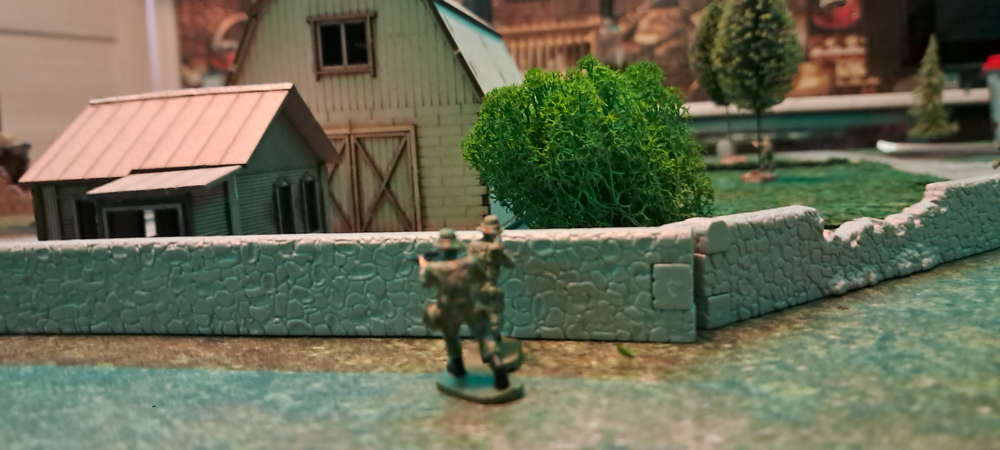
\includegraphics[width=\linewidth]{media/contract/image6.png}

\subsubsection{Маневрирование (МНВ)}\label{maneuver}

Навык определяет отработанные до автоматизма привычки, уменьшающие
площадь поражения тела до минимума. Человек умеет двигаться так, чтобы
свести к минимуму риск попадания под обстрел, постоянно оценивает
местность и держит в голове ближайшие естественные укрытия, своевременно
и оптимально меняет позы.

Высокий уровень навыка уменьшает вероятность поражения при стрельбе по
отряду.

При определении навыка маневрирования Ур(МНВ) отряда среди солдат отряда
выбирается минимальное значение.

\subsubsection{Маскировка (МСК)}\label{camouflage-skill}

Тренировки по маскировке включают в себя собственно маскировку, а также
обнаружение (демаскировку).
В ролевой части навык МСК используется во
взаимодействиях, связанных с восприятием и наблюдательностью.

Навык маскировки Ур(МСК) влияет на дальность обнаружения (демаскировки)
противника при наблюдении.

Игрок самостоятельно выбирает персонажа, который ведёт наблюдение,
поэтому применяется значение навыка Ур(МСК) конкретного персонажа, а
также учитывается экипировка, время суток и погодные условия. При
определении навыка маскировки Ур(МСК) отряда, за которым ведётся
наблюдение, выбирается минимальное значение среди персонажей этого
отряда.

\subsubsection{Навыки меткости}\label{weapon-skills}

Навыки, связанные с атрибутом меткость используются для определения
результативности применения оружия прямой наводкой, в том числе бросков
гранат.

Снаряжение и оружие делится на классы, для каждого из которых необходима
отдельная тренировка.

\subsubsection{Медицина (МЕД)}\label{medicine}

Навык медицины позволяет спасти жизнь смертельно раненого солдата и
остановить кровотечение. В ролевой части навык медицины используется во
взаимодействиях, связанных с медициной в целом, анатомией, биологией.

Санитару или медику, то есть персонажу с количеством очков навыка МЕД
больше 0, доступно оказание первой
помощи.

\subsubsection{Механика (МЕХ)}\label{mechanics}

Навык механики определяет возможности по ремонту и созданию различных
механизмов, а также по управлению ими. Навык может использоваться для
физического взлома и ремонта замков, автомобилей, а также для проверок
при управлении автомобилями и боевыми машинами.

\subsubsection{Электроника (ЭЛ)}\label{electronics}

Навык работы с компьютерами, включающий и программную, и аппаратную
части: программирование, пайка, электрические схемы. Используется для
работы со средствами связи, радиооборудованием.

\subsubsection{Взрывные устройства и мины (ВЗР)}\label{explosives}

Навык работы с взрывчатыми веществами и взрывными устройствами,
минами. Используется для создания и установки взрывных устройств и
разминирования.

\subsubsection{Огневая поддержка (ОП)}\label{fire-support}

Используется для любой навесной стрельбы (стрельбы непрямой наводкой)
начиная от подствольных гранатомётов и АГС и заканчивая ствольной
артиллерией и РСЗО.

\subsubsection{Логика (ЛГК)}\label{logic}

Навык логики используется при взаимодействии с другими персонажами.

В ролевой части логика используется для убеждения. Убедить можно только
в том, что сам персонаж считает правдой и в чём уверен.

Очки навыка ЛГК зависит от образования: 2 для школьника, 6 для среднего
специального образования, 8 для оконченного высшего, 11 для нескольких
высших, 15 для кандидата наук, 19 для доктора наук.

\subsubsection{Влияние (ВЛН)}\label{influence}

Навык влияния используется при взаимодействии с другими персонажами.

В ролевой части влияние используется для обаяния, запугивания и обмана.

Персонаж имеет характер, который определяет его стиль общения:

\begin{itemize}
\item
  Жёсткий: персонаж не может использовать обаяние; получает бонус +5 к
  влиянию при применении запугивания и обмана.
\item
  Гибкий: персонаж гибко подстраивается под ситуацию.
\item
  Мягкий: персонаж не может использовать запугивание и обман; получает
  бонус +5 к влиянию при применении обаяния.
\end{itemize}

\section{Создание персонажей}\label{character-creation}

В зависимости от желания игроков и уровня их опыта в ролевых играх вообще и с системой Контракт в частности, предлагается несколько вариантов начала игры:

\begin{enumerate}
\def\labelenumi{\arabic{enumi}.}
\item
  Создание гражданских персонажей с последующим прохождением обучения в учебном центре <<Мира и процветания>>. Это может быть интерактивное создание персонажа с гейм-мастером через заполнение анкеты, либо гейм-мастер может создать случайного гражданского здорового персонажа уровней чернорабочий, прораб или специалист (см. \autoref{table-char-gen})).
\item
  Создание военных персонажей и начало игры сразу на базе <<Мира и процветания>> в Белизе. Гейм-мастер может создать случайного здорового персонажа, прошедшего военные сборы уровня от мл. сержант до лейтенант (см. \autoref{table-char-gen}).
\item
  Подготовленные игроки могут создать персонажа самостоятельно, распределив 40 очков тренированности по любым навыкам для старта на базе <<Мира и процветания>>.
\end{enumerate}

Каждый персонаж может взять с собой сотовый телефон и \$100 в Белиз. Остальное снаряжение --- по согласованию с мастером или уже на месте.

\subsubsection{Создание случайного персонажа}\label{char-gen}

Начните с определения характера персонажа: эмоциональный и харизматичный или рациональный и интеллектуальный.
Это можно сделать под предпочитаемый игроком отыгрыш, либо просто подбросив монетку.

Определите примерный возраст и социальный уровень персонажа, ориентируйтесь на данные в таблице ниже.
Социальный уровень в сочетании с характером позволит определить очки навыка ЛГК или ВЛН.

Имеющие актуальный боевой опыт персонажи получают 8 ВНС, 4 МНВ, 1 МСК, 5 ЛС и 2 ГРН.
Гражданские персонажи могут выбрать только один навык от меткости, а остальные выбрать от других атрибутов.

В зависимости от уровня, персонаж получает возможность выбора нескольких навыков:
отдельно для навыков, связанных с атрибутом меткость, и отдельно для остальных навыков.
Их можно выбрать случайно или по желанию. Для каждого выбранного навыка определяется значение очков тренированности навыка, случайно или по желанию.

\setlength\rotheadsize{2.3cm}
\begin{minipage}{\columnwidth}
\small
\begin{talltblr}[
  caption = {Создание случайного персонажа},
  label = {table-char-gen}
]{
  hlines,
  row{odd}={fg=navy},
  row{even}={fg=black},
  colspec={Q[c,m,co=3]Q[c,m,co=1]Q[c,m,co=1]Q[c,m,co=1]Q[c,m,co=1]}
}
Уровень & \rothead{$\text{Макс}(\text{ЛГК}/\text{ВЛН})$} & \rothead{Количество\\навыков} & \rothead{Количество\\навыков\\меткости} & \rothead{Макс\\значение\\навыка} \\
{Рядовой\\Чернорабочий} & 2 & 1 & 1 & 10 \\
{Мл. сержант} & 4 & 1 & 2 & 20 \\
{Сержант\\Прораб} & 6 & 2 & 2 & 20 \\
{Лейтенант\\Специалист} & 8 & 2 & 1 & 14 \\
{Капитан\\Руководитель проекта} & 11 & 3 & 3 & 14 \\
{Майор\\Руководитель отдела} & 14 & 4 & 3 & 14 \\
{Полковник\\Директор департамента} & 17 & 4 & 3 & 10 \\
Генерал & 20 & 5 & 3 & 6 \\
\end{talltblr}
\end{minipage}

\subsection{Создание персонажа с помощью анкеты}\label{questionnaire-character}

\subsubsection{Предыстория}\label{intro-scenario}

Вам всегда казалась скучной рутина жизни? Дом-работа, поел --- сходил в туалет --- поспал. Нет никакой разницы между начальниками или клиентами: везде полно дураков, и тот факт, что они платят вам деньги за общение с ними, никак не может это компенсировать.

Другое дело --- красочная жизнь супергероя, спасающего весь мир, или хотя бы искателя приключений. Незнакомые экзотические страны, опасности и испытания --- вы чувствуете, что это может вдохновить вас.

И вот в один прекрасный момент ваш взгляд цепляется за баннер крупной транснациональной компании <<Мир и процветание>>, привлекающей специалистов в команды, помогающие государствам в борьбе с преступностью. Вы соблазняетесь заявленным уровнем дохода и дополнительными бонусами и решаетесь позвонить по указанному телефону.

Вас приглашают на встречу, где обещают безусловный фуршет. Перед встречей вас просят распечатать небольшую анкету, заполнить её и принести с собой. Вы понимаете, что это не обычная туристическая поездка, но полагаете, что сможете узнать на встрече все подробности и после этого решить для себя, подойдёт ли вам такое приключение.

Вы приходите на встречу, организованную в большой переговорной комнате в богатом офисе, расположенном в самом центре вашего города. Помимо вас на этой встрече ещё человек двадцать слушателей.

Привлекательные и аккуратные ассистенты собирают у слушателей опросники, после чего предлагают присаживаться на кресла, установленные рядами в центре зала.

Выступает представитель компании: аккуратно выбритый и подстриженный мужчина в гражданском костюме: брюках и пиджаке, но без галстука. На лацкане его пиджака металлический значок с эмблемой <<Мира и процветания>>. Он представляется как Антон Григорьев и начинает презентацию.

Компания <<Мир и процветание>> существует уже 45 лет и специализируется на обеспечении правопорядка на разных направлениях по всему миру. Контракты заключаются с правительствами, корпорациями и международными организациями. В портфолио компании работа в Афганистане с 1980 года, в Ираке, Польше, Венгрии, Германии с 1991, в Ливии с 2011 года, в Сирии с 2014, в Казахстане с 2017, в Канаде с 2019, в Мексике с 2020, в Грузии, Армении и Турции с 2022, в Бразилии с 2024.

Сейчас компания набирает людей для пополнения команды, работающей в Белизе, с которым недавно был заключён контракт. На текущем этапе <<Мир и процветание>> работает в Белизе параллельно с местными службами: полицией, армией и пограничной службой. Задача компании --- показать свою эффективность и в ближайшем будущем полностью заменить существующие силовые структуры в стране, после чего они будут расформированы.

Основные задачи на текущий момент: несение пограничной службы, задержание подозреваемых и передача их местным властям. Эта работа требует определённых навыков, поэтому проводится месячная интенсивная подготовка в учебном центре компании. Во время подготовки есть возможность выбора дополнительных курсов. Некоторые задачи могут быть связаны с риском для жизни, но, если следовать указаниям командиров, то этот риск будет минимальным.

Контракт с компанией можно заключить на разный срок, от 3 месяцев до нескольких лет. Но короткие сроки контракта доступны только для опытных специалистов, которые ранее уже работали с компанией, потому что в противном случае нужно будет пройти подготовку, и тогда компании не выгодно заключать контракт на короткий срок. У сотрудников компании после успешного прохождения подготовки есть возможность влиять на тактические решения, а также возможность занять командирские должности.

Компания <<Мир и процветание>> декларирует соблюдение законов и обычаев страны, в которой работает, всегда остаётся на стороне клиента и дорожит своей репутацией.

Компания использует всё своё влияние для помощи своим сотрудникам и после завершения контракта, потому что уверена, что бывших сотрудников не бывает. Построив с компанией доверительные отношения, вы можете получить протекторат по завершению контракта, который поможет вам получить серьёзное преимущество как в ведении собственного бизнеса, так и в движении по карьерной лестнице.

Затем ведущий приглашает гостей пройти на фуршет. Вы общаетесь с ведущим, с другими гостями и чувствуете, что преимущества контракта в ваших мыслях перевешивают кажущиеся маловероятными риски.

После фуршета, когда гостям предлагается принять решение и подписать документы, вы, уже особо не колеблясь, берёте контракт, присаживаетесь за стол и перечитываете его. Перед вами лежит авторучка. Контракт содержит пункт о неразглашении, уведомление о рисках для жизни и здоровья и пункты об ответственности за нарушение дисциплины и уже подписан директором компании, Джонатаном Энтони Келли. Вы берёте ручку, подписываете каждую страницу документа, и отдаёте документ ассистенту. В обмен тот передаёт вам карточку, где указано место и время посадки на транспорт для отправления в учебный центр.

\end{multicols}

\clearpage

\noindent
\includegraphics[width=4cm]{media/pap_players_book/image11.png}\hfill\colorbox{white}{\parbox[b][3cm][c]{3cm}{\centering\vspace*{0.2cm}Место для фото\vspace*{0.2cm}}}

\section{Анкета кандидата}\label{candidate-questionnaire}

\begin{enumerate}
\def\labelenumi{\arabic{enumi}.}
\item
  Имя, фамилия, отчество:\fillinline{}
\item
  Дата рождения:\fillinline{}
\item
  Должность на последнем месте работы:\fillinline{}

  {\scriptsize\rightline{(для руководителей указать кол-во подчинённых)}}
\item
  Свободное владение иностранными языками:\fillinline{}
\item
  Знания и опыт в медицине:\fillinline{}

  {\scriptsize\rightline{(навыки первой помощи/практикующий врач --- указать специализацию)}}
\item
  Навыки управления и обслуживания техники:\fillinline{}

  {\scriptsize\rightline{(категория вод. удостоверения, наличие автомобиля, курсы)}}
\item
  Опыт в обращении с оружием:\fillinline{}

  {\scriptsize\rightline{(курсы, лицензии, разрешения, спортивные звания)}}
\item
  Прохождение срочной службы:\fillinline{}

  {\scriptsize\rightline{(место, период прохождения, военная специальность)}}
\item
  Спортивные достижения:\fillinline{}

  {\scriptsize\rightline{(спортивное звание, частота тренировок)}}
\item
  Характерные черты:\fillinline{}

  {\scriptsize\rightline{(личные особенности)}}
\end{enumerate}

Я подтверждаю, что все данные мною в анкете ответы верны и содержат полную информацию, которая известна мне по сути заданных вопросов.

Я предупрежден, что в случае заключения со мной контракта, неверная информация, сообщенная мною в анкете, будет являться основанием для расторжения со мной контракта без выплаты компенсации.

Дата:\fillinline{}Подпись:\fillinline{}Расшифровка:\fillinline{}

\clearpage

\begin{multicols}{2}
\raggedcolumns{}

\section*{Краткая памятка}\label{quick-reference}
\addcontentsline{toc}{section}{Краткая памятка}

\subsection*{Что можно делать?}\label{what-can-be-done}
\addcontentsline{toc}{subsection}{Что можно делать?}

\subsubsection*{Отряд в целом}\label{squad-as-a-whole}

\begin{itemize}
\item
  Изменить состав отряда --- разделиться/объединиться.
\item
  Идти, бежать, перелезать забор, сесть в технику, выйти из техники, зайти в здание, выйти из здания.
\item
  Штурмовать и захватывать в плен в бою (при сближении вплотную).
\end{itemize}

\subsubsection*{Отдельные персонажи}\label{individual-characters}

\begin{itemize}
\item
  Для экипажа: управлять техникой, вести огонь из вооружения техники.
\item
  Ремонтировать технику --- проверка на механику.
\item
  Наблюдать (можно указать конкретное направление или место), в том числе с использованием экипировки.
\item
  Использовать вооружение (целиться из снайперской винтовки, разворачивать и сворачивать миномёт, вести огонь, метать гранаты, ставить и обезвреживать мины).
\item
  Говорить лично/по рации.
\item
  Осмотреть предмет, конструкцию, локацию, подбирать/передавать/выбрасывать предметы.
\item
  Оказать первую помощь раненому (или самому себе) --- проверка на медицину.
\item
  Обмануть, убедить, угрожать --- проверка на лидерство.
\item
  Рукопашный бой, толкнуть, схватить --- проверка на физическую подготовку.
\item
  Другие заявки --- на усмотрение мастера.
\end{itemize}

\subsection*{Что влияет на результат стрельбы?}\label{what-affects-shooting}
\addcontentsline{toc}{subsection}{Что влияет на результат стрельбы?}

\begin{itemize}
\item
  Идентификация цели --- насколько хорошо отряд, ведущий огонь наблюдает цель. Видна ли она стрелку непосредственно или огонь ведётся вслепую?
\item
  Качество прицеливания (усталость, удобство позиции, время на прицеливание).
\item
  Навык использования конкретного оружия стрелка --- Ур(ОРУЖ), а также характеристики оружия.
\item
  Если цель --- пехота, то учитывается Ур(ТП) цели; можно получить бонус при обстреле отряда пехоты с разных сторон.
\item
  Если цель --- техника, то учитывается её уровень бронированности и место попадания (в лоб, в корму, в борт).
\item
  Расстояние между целью и стрелком.
\item
  Качество позиции (укрытия) цели.
\end{itemize}

\subsection*{На что влияют навыки?}\label{what-skills-affect}

\subsubsection*{Лидерство}\label{leadership-skill-summary}
\addcontentsline{toc}{subsubsection}{Лидерство}

Быстрее восстановление от стресса, выше инициатива (приоритет действия), больше персонажей в отряде, больше отрядов под руководством.

\subsubsection*{Физическая подготовка}\label{fitness-skill-summary}
\addcontentsline{toc}{subsubsection}{Физическая подготовка}

Больше грузоподъёмность, выше скорость, выше выносливость. Грузоподъёмность персонажей суммируется в отряде. Перемещение шагом: от 2 см до 5 см за ход шагом в зависимости от нагрузки. Перемещение бегом: в 2 раза быстрее, чем шагом, но требует увеличения очков усталости; не более Ур(ФП) очков усталости, при этом выбирается минимальное значение Ур(ФП) из персонажей в отряде.

\subsubsection*{Тактическая подготовка}\label{tactics-skill-summary}
\addcontentsline{toc}{subsubsection}{Тактическая подготовка}

Уменьшает вероятность поражения при стрельбе по отряду. Выбирается минимальный Ур(ТП) среди персонажей отряда, по которому ведётся стрельба!

\subsubsection*{Медицина}\label{medicine-skill-summary}
\addcontentsline{toc}{subsubsection}{Медицина}

Позволяет сохранить жизнь персонажу, истекающему кровью.\\
Модификатор броска при оказании помощи: +Ур(МЕД), сложность 12+.

\subsubsection*{Маскировка}\label{camouflage-skill-summary}
\addcontentsline{toc}{subsubsection}{Маскировка}

Все отряды начинают игру замаскированными. Для того, чтобы заметить отряд противника, необходимо выполнять наблюдение и проходить проверку с броском кубика. При стрельбе по неидентифицированному замаскированному противнику модификтор броска стрельбы -6!

Высокий навык маскировки позволяет лучше скрываться, лучше обнаруживать мины и засады и лучше прятать ловушки. Выбирается минимальный Ур(МСК) среди персонажей в отряде, за которым ведётся наблюдение!

\subsubsection*{Навыки владения оружием}\label{weapon-skills-summary}
\addcontentsline{toc}{subsubsection}{Навыки владения оружием}

Отдельно для каждого типа оружия.\\
Увеличивает шансы поразить цель этим оружием. Навык <<взрывные устройства и мины>> влияет также на успех при обезвреживании взрывных устройств.

\subsubsection*{Навыки в механике (владения техникой)}\label{mechanic-skills-summary}
\addcontentsline{toc}{subsubsection}{Навыки в механике (владения техникой)}

Отдельно для автомобилей, колёсных вездеходов и гусеничных вездеходов. Позволяет управлять этим типом техники при ненулевом уровне. При управлении Ур(МЕХ) влияет на преодоление препятствий и сохранение контроля на высоких скоростях. При ремонте можно использовать навык МЕХ для любого типа техники, но, если тип не соответствует, значение МЕХ делится на два.

\end{multicols}

\clearpage

\section*{Лист отряда}\label{squad-sheet}
\addcontentsline{toc}{section}{Лист отряда}

\noindent
\begin{talltblr}[
  caption = {},
  label = {table-squad-sheet}
]{
  hlines,
  colspec={Q[l,m,co=3]Q[l,m,co=1]Q[l,m,co=1]},
  cell{1}{1}={c=5}{c},
  row{1}=
{ht=2cm}
}
\SetCell{c,m} \textbf{Лист отряда} \\
& & & & \\
\end{talltblr}

Позывной: \rule{8cm}{0.4pt}

\subsection*{Навыки}\label{skills-summary}
\addcontentsline{toc}{subsection}{Навыки}

\subsubsection*{Уровни}\label{skill-levels}
\addcontentsline{toc}{subsubsection}{Уровни}

\begin{center}
\begin{minipage}{0.9\columnwidth}
\small
\begin{talltblr}[
  caption = {Уровни навыков},
  label = {table-skill-levels-summary}
]{
  hlines,
  row{odd}={fg=navy},
  row{even}={fg=black},
  colspec={Q[c,m,co=1]Q[c,m,co=1]Q[c,m,co=1]Q[c,m,co=1]Q[c,m,co=1]Q[c,m,co=1]Q[c,m,co=1]},
}
Уровень навыка Ур(X) & 1 & 2 & 3 & 4 & 5 & 6 \\
Очки навыка X & 1+ & 3+ & 7+ & 12+ & 16+ & 20+ \\
\end{talltblr}
\end{minipage}
\end{center}

\subsubsection*{Навыки персонажа}\label{character-skills}
\addcontentsline{toc}{subsubsection}{Навыки персонажа}

\begin{minipage}{\columnwidth}
\small
\begin{talltblr}[
  caption = {Навыки персонажа},
  label = {table-character-skills}
]{
  hlines,
  row{odd}={fg=navy},
  row{even}={fg=black},
  colspec={Q[l,m,co=2]Q[c,m,co=1]},
}
Лидерство (ЛИД) & Очки/уровень \\
Физическая подготовка (ФП) & \\
Тактическая подготовка (ТП) & \\
Медицина (МЕД) & \\
Маскировка (МСК) & \\
Гранаты (метательное) & \\
Лёгкое стрелковое & \\
Пулемёты & \\
Снайперское & \\
Гранатомёты & \\
Реактивные гранатомёты & \\
Противотанковые ракетные комплексы & \\
Миномёты & \\
Беспилотные летательные аппараты & \\
Взрывные устройства и мины & \\
Переносные зенитно-ракетные комплексы & \\
Автоматические пушки & \\
Танковые орудия & \\
Артиллерийские системы & \\
Ракетные системы залпового огня & \\
Автомобили (МЕХ) & \\
Колёсные боевые машины (МЕХ) & \\
Гусеничные боевые машины (МЕХ) & \\
\end{talltblr}
\end{minipage}

\subsubsection*{Снаряжение}\label{equipment}
\addcontentsline{toc}{subsubsection}{Снаряжение}

\begin{minipage}{\columnwidth}
\small
\begin{talltblr}[
  caption = {Снаряжение},
  label = {table-equipment}
]{
  hlines,
  row{odd}={fg=navy},
  row{even}={fg=black},
  colspec={Q[l,m,co=2]Q[l,m,co=1]},
}
Предмет, вес & Боезапас, вес \\
& \\
& \\
& \\
& \\
& \\
& \\
& \\
& \\
& \\
& \\
& \\
& \\
& \\
& \\
& \\
& \\
& \\
\end{talltblr}
\end{minipage}

\subsection*{Заметки}\label{notes}
\addcontentsline{toc}{subsection}{Заметки}

\vspace{10cm}

\end{document}
